\clearpage\begingroup\SourceLeaf{101}\HistoricalHead{96}{L}{PHYSIK. BRIEFWECHSEL.}
\begin{center}[15.]\end{center}
\begin{center}\textsc{Gauss} an \textsc{Gerling}.\quad Göttingen, 4. December 1834.\end{center}
\noindent .\ .\ .\ .\ .\ .\ .\ .\ .\ .\ .\ .\ .\ .\ .\ .\ .\ .\ .\ .\ .
\par\noindent\hspace*{\parindent}Einer der früheren Apparate von 1832 (einpfündige Nadel) ist jetzt im
Phys. Kabinet aufgestellt, nebst dem Multiplicator von 68 Windungen, 300
Fuss Drahtlänge. Der Apparat im M[agnetischen] O[bservatorium] hat einen
Multiplicator von 200 Windungen, 1100 Fuss Drahtlänge. Seit Julius habe
ich in der Sternwarte eine \textls[120]{25pfündige} Nadel aufgehängt, woran die Beobb.
eine bewundernswürdige Harmonie geben; seit 6 Wochen hat auch diese Nadel
ihren Multiplicator von 270 Windungen, 2700 Fuss Drahtlänge. Alle drei Apparate
sind in Einer galvanischen Kette verbunden; ganze Drahtlänge die Multiplicatoren
mitgerechnet 11000---12000 Fuss. Die Versuche damit öffnen ein
ganz neues Feld zu Resultaten in scharfen quantitativen Verhältnissen. Die
Unmessbarkeit der Zeit, in der der Strom durchlaufen wird, ist bereits oft
constatirt; wir vergleichen die Uhren dadurch auf einen kleinen Bruch der
Secunde genau. Die Stärke des Stroms ist an allen Stellen dieselbe, ein
höchst wichtiges Resultat, dessen Zulässigkeit \textls[120]{während Regens} jedoch erst
noch geprüft werden wird. Am allerinteressantesten sind mir die Inductionsversuche,
wozu eine Rolle mit 1026 Drahtumwindungen da ist (die ich vielleicht
voriges Jahr Ihnen schon gezeigt habe). Ein Wechsel von
\par\nopagebreak\begin{center}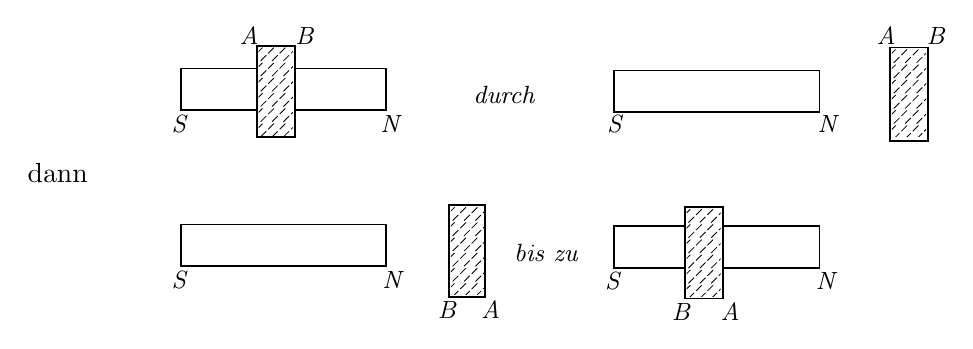
\begin{tikzpicture}[x=.0095in,y=-.0095in,line width=.65pt]
\draw (90,22)--(50,22)--(50,44)--(90,44) (110,22)--(158,22)--(158,44)--(110,44);
\draw (90,10) rectangle (110,58);
\draw (278,23) rectangle (386,45);
\draw (423,11) rectangle (443,60);
\draw (50,104) rectangle (158,126);
\draw (191,94) rectangle (210,142);
\draw (315,105)--(278,105)--(278,127)--(315,127) (335,105)--(386,105)--(386,127)--(335,127);
\draw (315,95) rectangle (335,143);
\foreach \a/\b in {90/10,423/11,191/94,315/95}{
  \begin{scope}[shift={(\a,\b)}]
  \clip (1,1) rectangle (19,47);
  \draw[line width=.3pt]
  (0,4)--(3,1) (6,4)--(9,1) (12,4)--(15,1) (18,4)--(21,1)
  (2,8)--(5,5) (8,8)--(11,5) (14,8)--(17,5)
  (0,12)--(3,9) (6,12)--(9,9) (12,12)--(15,9) (18,12)--(21,9)
  (2,16)--(5,13) (8,16)--(11,13) (14,16)--(17,13)
  (0,20)--(3,17) (6,20)--(9,17) (12,20)--(15,17) (18,20)--(21,17)
  (2,24)--(5,21) (8,24)--(11,21) (14,24)--(17,21)
  (0,28)--(3,25) (6,28)--(9,25) (12,28)--(15,25) (18,28)--(21,25)
  (2,32)--(5,29) (8,32)--(11,29) (14,32)--(17,29)
  (0,36)--(3,33) (6,36)--(9,33) (12,36)--(15,33) (18,36)--(21,33)
  (2,40)--(5,37) (8,40)--(11,37) (14,40)--(17,37)
  (0,44)--(3,41) (6,44)--(9,41) (12,44)--(15,41) (18,44)--(21,41)
  (2,48)--(5,45) (8,48)--(11,45) (14,48)--(17,45);
  \end{scope}}
\foreach \a/\b/\c in {86/5/A,115/5/B,49/51/S,160/51/N,421/5/A,447/5/B,278/51/S,390/51/N,49/133/S,161/133/N,190/149/B,213/149/A,277/134/S,389/134/N,313/150/B,339/150/A}
  \node[inner sep=0pt,font=\small\itshape] at (\a,\b) {\c};
\node[font=\small\itshape] at (220,36) {durch};
\node[anchor=west,inner sep=0pt] at (-31,77) {dann};
\node[font=\small\itshape] at (242,119) {bis zu};
\end{tikzpicture}
\end{center}
\noindent den man in \(1''\) bis \(2''\) machen kann, bringt einen galvanischen Strom in die mit
den Enden des Rollendrahtes verbundene Kette, der, wenn er durch die \textls[120]{ganze}
Kette geht, eine Bewegung von 11 Scalentheilen hervorbringt; und da mit
dem Commutator (alias Gyrotrop) die entgegengesetzte Bewegung der Rolle \textls[120]{zu}
\textls[120]{gleichem} Strom verwandt werden kann, so bringt man in kurzer Zeit die
\clearpage\SourceLeaf{102a}\HistoricalHead{97}{R}{GAUSS AN GERLING UND OLBERS.}
\noindent ganze Scale aus dem Felde. Am Apparat der 4 pf. Nadel des\linebreak M[agnetischen]
O[bservatoriums] beträgt die Wirkung desselben Manövers \(2\frac{1}{2}\)mahl so viel.
Diese Versuche, womit ich jetzt beschäftigt bin, sind um so interessanter, da
sie sehr scharfe Resultate zu geben fähig sind, was bei rein galvanischen,
wegen der Veränderlichkeit der electromotorischen Kraft und des Widerstandes
nur bedingungsweise der Fall ist. Doch habe ich auch in Beziehung auf
letztere schon überaus interessante Resultate gefunden. Ein Commutator von
einer anderen Einrichtung ist jetzt bei \textsc{Meierstein} in Bestellung gegeben und
wird in Kürze fertig sein. Mit diesen und einigen andern Abänderungen
hoffe ich binnen Einer Secunde \textls[120]{zwei vollständige} Wechsel machen und
dadurch die betreffenden Zahlen mit äusserster Schärfe bestimmen zu können.
\par\noindent .\ .\ .\ .\ .\ .\ .\ .\ .\ .\ .\ .\ .\ .\ .\ .\ .\ .\ .\ .\ .
\clearpage\endgroup
